\documentclass[12pt]{article}
\usepackage[a4paper]{geometry}

\usepackage[utf8]{inputenc}
\usepackage[T2A]{fontenc}

\usepackage[russian]{babel}

\usepackage{mathtools}
\usepackage{bm}
\usepackage{IEEEtrantools}

\usepackage{minted}

\usepackage{tabu}
% `footnotes` fixes footnotes issues in tables
\usepackage{footnote}

\usepackage{graphicx}
\usepackage{subcaption}
% set up graphicx to use custom path to graphs
\graphicspath{{graphs/}}

% make indentation at the beginning of sections
\usepackage{indentfirst}

% backend=biber is the default but /wo it there is a warning
% use the biblatex-gost package which provides gost support
\usepackage[backend=biber,bibstyle=gost-standard]{biblatex}
\bibliography{references}

% set a couple mathematical environments
\newtheorem{definition}{Определение}
\newtheorem{example}{Пример}

\DeclareMathOperator*{\argmin}{arg\,min}
\DeclareMathOperator*{\argmax}{arg\,max}

\usepackage[norelsize,ruled,vlined]{algorithm2e}
%\usepackage[all]{xy}

% do not show colored borders around links
\usepackage[hidelinks]{hyperref}

% Параметры страницы
%% \textheight=24cm
%% \textwidth=16cm
%% \oddsidemargin=5mm
%% \evensidemargin=-5mm
%% \marginparwidth=36pt
%% \topmargin=-1cm
%% \flushbottom
%% \raggedbottom
%% \tolerance 3000
%% % подавить эффект "висячих стpок"
%% \clubpenalty=10000
%% \widowpenalty=10000
\renewcommand{\baselinestretch}{1.1}
%% \renewcommand{\baselinestretch}{1.5} %для печати с большим интервалом

\begin{document}

\begin{titlepage}
\begin{center}
    Московский государственный университет имени М. В. Ломоносова

    \bigskip
    
\includegraphics[width=50mm]{msu.eps}

    \bigskip
    Факультет Вычислительной Математики и Кибернетики\\
    Кафедра Математических Методов Прогнозирования\\[10mm]

    \textsf{\large\bfseries
        ВЫПУСКНАЯ КВАЛИФИКАЦИОННАЯ РАБОТА \\СТУДЕНТА 417 ГРУППЫ\\[10mm]
        <<Обработка множеств логических закономерностей с помощью
        дисперсионного критерия>>
    }\\[10mm]

    \begin{flushright}
        \parbox{0.5\textwidth}{
            Выполнил:\\
            студент 4 курса 417 группы\\
            \emph{Лисяной Александр Евгеньевич}\\[5mm]
            Научный руководитель:\\
            д.ф-м.н., профессор\\
            \emph{Рязанов Владимир Васильевич}
        }
    \end{flushright}

    \begin{tabular}{p{0.45\textwidth}p{0.45\textwidth}}
        Заведующий кафедрой\newline
        Математических Методов\newline
        Прогнозирования, академик РАН
        &
        ~\newline~\newline
        \hfill\hbox to 0.45\textwidth{\hrulefill~Ю. И. Журавлёв}
    \\[20mm]
        К защите допускаю\newline
        \hbox to 0.4\textwidth{<<\hbox to 12mm{\hrulefill}>> \hrulefill~2015 г.}
        &
        К защите рекомендую\newline
        \hbox to 0.45\textwidth{
          <<\hbox to 12mm{\hrulefill}>> \hrulefill~2015 г.
        }
    \end{tabular}

    \vspace{\fill}
    Москва, 2015
\end{center}
\end{titlepage}

\newpage
\renewcommand{\contentsname}{Содержание}
\tableofcontents

\newpage
\begin{abstract}
  %% Данный документ является образцом оформления дипломной работы
  %% для студентов кафедры Математических методов прогнозирования
  %% ВМК~МГУ. Приведённые ниже рекомендации взяты из~статьи
  %% <<Написание отчётов и статей (рекомендации)>> на~вики"~ресурсе
  %% \texttt{www.MachineLearning.ru}.  Студенты, готовящие дипломную
  %% работу к~защите, могут найти много полезной информации также
  %% в~статьях <<Научно-исследовательская работа (рекомендации)>>,
  %% <<Подготовка презентаций (рекомендации)>>, <<Защита выпускной
  %% квалификационной работы (рекомендации)>> на~том~же ресурсе.

  %% Аннотация обычно содержит краткое описание постановки задачи
  %% и~полученных результатов, одним абзацем на 10--15 строк.  Цель
  %% аннотации "--- обозначить в~общих чертах, о~чём работа, чтобы
  %% человек, совершенно не~знакомый с~данной работой, понял,
  %% интересна~ли ему эта тема, и~стоит~ли читать дальше. Аннотация
  %% собирается в~последнюю очередь путем легкой модификации наиболее
  %% важных и~удачных фраз из введения и~заключения.

  Одной из основных задач машинного обучения является задача
  классификации. Существует множество разнообразных алгоритмов
  классификации, в том числе алгоритмы, основанные на поиске
  логических закономерностей в данных. Этот поиск --- довольно
  трудоемкая задача. Приходится прибегать к различного рода
  эвристикам, то есть как-то ограничивать время работы полного
  перебора. Полученные логические закономерности могут оказаться
  слишком сложными (переобученными) или очень похожими (не
  \emph{диверсифицированными}). Поэтому, как правило, применяются
  различные методы обработки множества логических
  закономерностей. Целью данной работы является реализовать и
  применить метод обработки множества логических закономерностей с
  помощью дисперсионного критерия к результату работы алгоритма
  <<логические закономерности>>, реализованного в системе
  <<Распознавание>>.

\end{abstract}

\newpage
\section{Введение}
%% Во введении рассказывается, где возникает данная задача, и~почему её
%% решение так важно. Вводится на неформальном уровне минимум терминов,
%% необходимый для понимания постановки задачи.  Приводится краткий
%% анализ источников информации (литературный обзор): как эту задачу
%% решали до сих пор, в~чем недостаток этих решений, и~что нового
%% предлагает автор. Формулируются цели исследования. В~конце введения
%% даётся краткое содержание работы по разделам; при этом отмечается,
%% какие подходы, методы, алгоритмы предлагаются автором впервые.
%% При~упоминании ключевых разделов кратко формулируются основные
%% результаты и~наиболее важные выводы.

%% Цель введения: дать достаточно полное представление о~выполненном
%% исследовании и~полученных результатах, понятное широкому кругу
%% специалистов. Большинство читателей прочтут именно введение и, быть
%% может, заключение.

%% Во~введении автор решает сложную оптимизационную проблему: как
%% сообщить только самое важное, потратив минимум времени читателя,
%% да~так, чтобы максимум читателей поняли, о~чём вообще идёт речь.

%% Введение лучше писать напоследок, так как в~ходе работы обычно
%% происходит переосмысление постановки задачи.Если же введение писать,
%% когда работа еще не~готова, задача усложняется вдвойне.  В~конце
%% обычно приходит понимание, что всё получилось совсем не~так, как
%% планировалось в~начале, и~исходный вариант всё равно придётся
%% переписывать. Кстати, к~таким «потерям» надо относиться спокойно~---
%% в~хорошей работе почти каждый абзац многократно переделывается
%% до~неузнаваемости.

%% Введение имеет много общего с~текстом доклада на~защите, поэтому
%% имеет смысл готовить их одновременно.

Одной из основных задач машинного обучения является задача
классификации. Существует множество разнообразных алгоритмов
классификации, в том числе алгоритмы, основанные на поиске логических
закономерностей в данных. Результатом работы таких алгоритмов является
набор логических закономерностей (правил), используя которые можно
принимать решение о том, к какому классу принадлежит тот или иной
объект. Обычно такие правила имеют вид конъюнкции по всем признакам
объекта, где каждый терм конъюнкции представляет из себя допустимый
диапазон для значений признака, при котором объект может быть
\emph{покрыт} данным правилом.

Поиск логических закономерностей в данных --- довольно трудоемкая
задача. Каждый алгоритм использует различные предположения при
построении логических закономерностей. Например, алгоритм <<логические
закономерности>>, реализованный в системе
<<Распознавание>>\cite{recognition06}, для каждого объекта обучающей
выборки производит перебор по всем значениям каждого отдельно взятого
признака. В результате такого перебора выбирается некоторое конкретное
значение признака, которое затем используется при построении
соответствующего терма конъюнкции. В итоге получается правило, которое
как бы <<натянуто>> на некоторые объекты обучающей выборки.

При построении логических закономерностей возникают разного рода
проблемы. Во-первых, количество правил может оказаться довольно
большим. Во-вторых, могут получаться вырожденные или очень похожие
друг на друга логические закономерности. Поэтому отдельный интерес
представляет задача по обработке полученных множеств логических
закономерностей. Эта задача заключается в том, чтобы по исходному
множеству логических закономерностей построить множество меньшей
мощности и сравнимым качеством классификации.

Целью данной работы является реализовать и применить метод обработки
множества правил, основанный на кластеризации с помощью дисперсионного
критерия, к результату работы алгоритма <<логические закономерности>>,
представленного в системе <<Распознавание>>. В этом методе
предлагается использовать описание логических закономерностей с
помощью вектора левых и правых границ и сравнить его с бинаризованным
описанием логических закономерностей, предложенным в
\cite{novikov15}. На шаге кластеризации в дисперсионном критерии
предлагается использовать <<вес>> для отделения более информативных
правил.

Обработанные множества логических закономерностей сравниваются как
между собой (в ходе обработки используются различные способы описания
правил и критерии информативности), так и с исходным множеством
логических закономерностей, полученным в результате настройки
алгоритма системы <<Распознавания>>. В результате предложенный в
данной работе подход с использованием вектора левых и правых границ и
взвешенной кластеризации в целом работает лучше, чем подход с
бинаризованным описанием из \cite{novikov15}. Качество
классификации сравнимо с исходным алгоритмом системы
<<Распознавание>>, но при этом размер множества логических
закономерностей меньше.

\subsection{Определения и~обозначения}
\label{subsec:defs}

%% Формальная постановка задачи. Для известных понятий желательно
%% придерживаться стандартных обозначений.

%% Общепринятые термины вводятся словом «называется». Термины,
%% придуманные самим автором, вводятся словами «назовём» или «будем
%% называть».  Обычно этот раздел заканчивается формальной постановкой
%% задачи.  Именно с~этого раздела стоит начинать писать работу.

% постановка задачи классификации Воронцовым
Основные определения и обозначения будем вводить согласно
\cite{voron10logicalgs}. Пусть имеется пространство объектов \(X\) и
конечное множество имен классов \(Y = \left\{1, \dots,
M\right\}\). Пусть также имеется \emph{обучающая выборка} \(X^{l} =
(x_i, y_i)_{i = 1}^{l}\), в которой для каждого объекта \(x_i\)
известен его класс \(y_i \in Y\).  Для восстановления целевой
зависимости \(y^{*}(x_i) = y_i\) построим алгоритм классификации
\(a\colon X \rightarrow Y\), аппроксимирующий \(y^{*}\) на всём
пространстве объектов \(X\).

Для решения такой задачи классификации (восстановления зависимости
\(y^{*}\) по обучающей выборке \(X^l\)) существует множество
разнообразных алгоритмов. Некоторые из них основаны на поиске
логических закономерностей.

\begin{definition}
  Функция \(\varphi(x) \colon X \rightarrow \left\{0, 1\right\}\)
  называется \emph{предикатом}. Говорят, что предикат
  \(\varphi\) \emph{выделяет} или \emph{покрывает} объект \(x \in X\),
  если \(\varphi(x) = 1\).
\end{definition}

Формализуем понятие \emph{закономерности} так, как сделано в
\cite{voron10logicalgs}. Для того введем несколько обозначений:

\begin{itemize}
\item Пусть \(P_c\) --- число объектов класса \(c\) в выборке \(X^l\).
\item Пусть \(p_c(\varphi)\) --- число объектов \(x\) класса \(c\), на
  которых \(\varphi(x) = 1\)
\item Пусть \(N_c\) --- число объектов всех остальных классов \(Y
  \setminus \left\{c\right\}\)
\item Пусть \(n_c(\varphi)\) --- число объектов \(x\) не из объектов
  класса \(c\), на которых \(\varphi(x) = 1\)
\item Обозначим долю ошибочно выделяемых объектов среди всех объектов,
  покрываемых \emph{закономерностью}, через \(E_c(\varphi, X^l) =
  \frac{n_c(\varphi)}{p_c(\varphi) + n_c(\varphi)}\)
\item Обозначим долю верно выделяемых объектов через \(D_c(\varphi,
  X^l) = \frac{p_c(\varphi)}{l}\)
\end{itemize}

\begin{definition}
  Предикат \(\varphi(x)\) называется
  \emph{\(\varepsilon\),\(\delta\)-закономерностью} для класса \(c \in
  Y\), если \(E_c(\varphi, X^l) \leq \varepsilon \) и \(D_c(\varphi,
  X^l)\geq\delta\) при заданных \(\varepsilon\) и \(\delta\) из
  отрезка \([0, 1]\)
\end{definition}

Такие \(\varepsilon\),\(\delta\)-закономерности также называют
\emph{логическими закономерностями}, \emph{закономерностями} или
\emph{правилами}.

Вообще говоря, предикаты \(\varphi(x)\colon X \rightarrow Y\) могут
иметь довольно сложный вид. Например, если в качестве объектов из
\(X\) выступают точки на числовой прямой, то для классификации на
рациональные и иррациональные числа можно взять аналог функции Дирихле
в качестве предиката:

\[
\varphi(x) =
\begin{dcases*}
1 & \(x \in \mathbf{Q}\) \\
0 & \(x \in \mathbf{R} \setminus \mathbf{Q}\)
\end{dcases*}
\]

Для того, чтобы предикаты были более простыми, введем
ограничение на их вид так, как было сделано в
\cite{ryazanov07logic}.

\begin{definition}
Пусть \(c_1, c_2 \in R\), \(f_j(x)\) --- j-ый признак объекта \(x\),
тогда \emph{параметрическим элементарным предикатом} будем
называть
\[
P^{c_1, c_2}(f_j(x)) =
\begin{dcases*}
1 & при \(c_1 \leq f_j(x) \leq c_2\) \\
0 & иначе
\end{dcases*}
\]
\end{definition}

Поскольку в предикате используется лишь один признак из всего
признакового описания объекта, то такой предикат называется
элементарным. Параметры \(c_1, c_2 \in R\) для каждого отдельного
признака \(f_j(x)\) выбираются, вообще говоря, свои, поэтому предикат
называют параметрическим.

Будем считать, что
\emph{логическая \(\varepsilon\),\(\delta\)-закономерность} \(\varphi(x)\)
имеет вид конъюнкции параметрических элементарных предикатов:
\begin{equation} \label{eq:parpred}
\varphi(x) = \land_{f_j(x)} P^{c_1^j, c_2^j}(f_j(x))
\end{equation}

Здесь индексы \(j\) над параметрами \(c_1^j, c_2^j\) означают, что для
каждого признака могут быть выбраны свои границы. Для логических
закономерностей такого вида есть простая геометрическая интерпретация
--- это построенные по объектам обучающей выборки \(X\) прямоугольные
гиперпараллелепипеды.


\section{Проблема поиска логических закономерностей}
%% Лучше, чтобы название этого подраздела было содержательным, например,
%% общепринятым названием задачи, проблемы или метода, рассматриваемого
%% в~данной работе.

%% Перечисляются подходы, методы, факты, на которые существенно опирается
%% данная работа, но~которые могут быть не~известны широкому кругу
%% читателей.  Здесь ссылки на литературу обязательны.  Теоремы только
%% формулируются, но не~доказываются.

%% Данный раздел преследует две цели.  Во-первых, сделать работу
%% самодостаточной~--- дать необходимый минимум информации тем читателям,
%% которые не~очень хорошо ориентируются в~теме, но желают поближе
%% познакомиться именно с~данной работой.  Во-вторых, облегчить
%% сопоставление полученных автором результатов с~ранее известными.

Поиск наиболее информативных логических закономерностей требует
определенных вычислительных затрат. Пусть множество \(\mathcal{P}\)
параметрических элементарных предикатов конечно. Тогда множество
\(\mathcal{K}_K\) логических закономерностей, состоящих не более, чем
из \(K\) термов, имеет вид:

\[
\mathcal{K}_K =
\left\{
 \varphi(x) = P_1(x) \& P_2(x) \& \dots \& P_k(x) \mid
  P_1, \dots, P_k \in \mathcal{P}, k \leq K
\right\}
\]

Количество логических закономерностей: \(\lvert \mathcal{K} \rvert =
\lvert \mathcal{P} \rvert^{K}\).

\subsection{Алгоритмы по созданию логических закономерностей}

К таким алгоритмам относятся <<КОРА>> \cite{vainzvaig73kora}, <<IREP>>
и <<RIPPER>> \cite{cohen95fast}, <<SLIPPER>> \cite{cohen99simple},
<<ID3>> \cite{quinlan86induction}, <<C4.5rules>>
\cite{quinlan93programs}, \cite{quinlan96bagging}.  В качестве
классического примера такого алгоритма можно привести двухклассовую
версию <<IREP>> [\ref{algo:IREP}].

\begin{algorithm}[!htpb]
  \caption{Incremental Reduced Error Pruning (IREP)}\label{algo:IREP}
  \SetKwInOut{Input}{Вход}\SetKwInOut{Output}{Выход}
  \Input{Pos --- множество элементов класса \(+1\) \newline
    Neg --- множество элементов класса \(-1\)
  }
  \Output{Rules --- множество правил}
  \SetKwFunction{IREP}{IREP}
  \SetKwProg{Fn}{Функция}{}{}
  \SetKwFor{While}{Пока}{}{}
  \SetKwIF{If}{Elif}{Else}{Если}{то}{Иначе если}{Иначе}{}
  \SetKw{KwRet}{Вернуть}
  \Fn{\IREP{Pos, Neg}} {
    Завести пустой набор правил Ruleset\;
    \While{Pos не опустеет}{
      \tcc{Нужно обучить и упростить очередное правило Rule}
      Разделить (Pos, Neg) на (GrowPos, GrowNeg) и (PrunePos, PruneNeg)\;
      Обучить правило Rule по паре множеств (GrowPos, GrowNeg)\;
      Упростить правило Rule по паре множеств (PrunePos, PruneNeg)\;
      \uIf{доля ошибок Rule на (PrunePos, PruneNeg) больше 50\%}{
        \KwRet{Ruleset}\;
      }
      \Else{
        Добавить правило Rule в Ruleset\;
        Убрать из (Pos, Neg) объекты, которые покрывает правило Rule\;
      }
    }
    \KwRet{Ruleset}\;
  }
\end{algorithm}

Алгоритм IREP [\ref{algo:IREP}] является одним из классических примеров
жадных алгоритмов построения правил, работающий по принципу <<разделяй
и властвуй>> (divide and conquer). Этот принцип проявляется в том, что
правила создаются по одному, а объекты, которые покрываются созданным
правилом, исключаются из рассмотрения. Многие алгоритмы (<<КОРА>>,
<<ТЭМП>> \cite{voron10logicalgs}) по смыслу очень похожи и отличаются
только критериями останова и способами упрощения полученных правил.

\subsection{Проблемы алгоритмов поиска логических закономерностей}

Многие алгоритмы поиска логических закономерностей имеют следующие
проблемы:

\begin{figure}[!htbp]
  \centering
  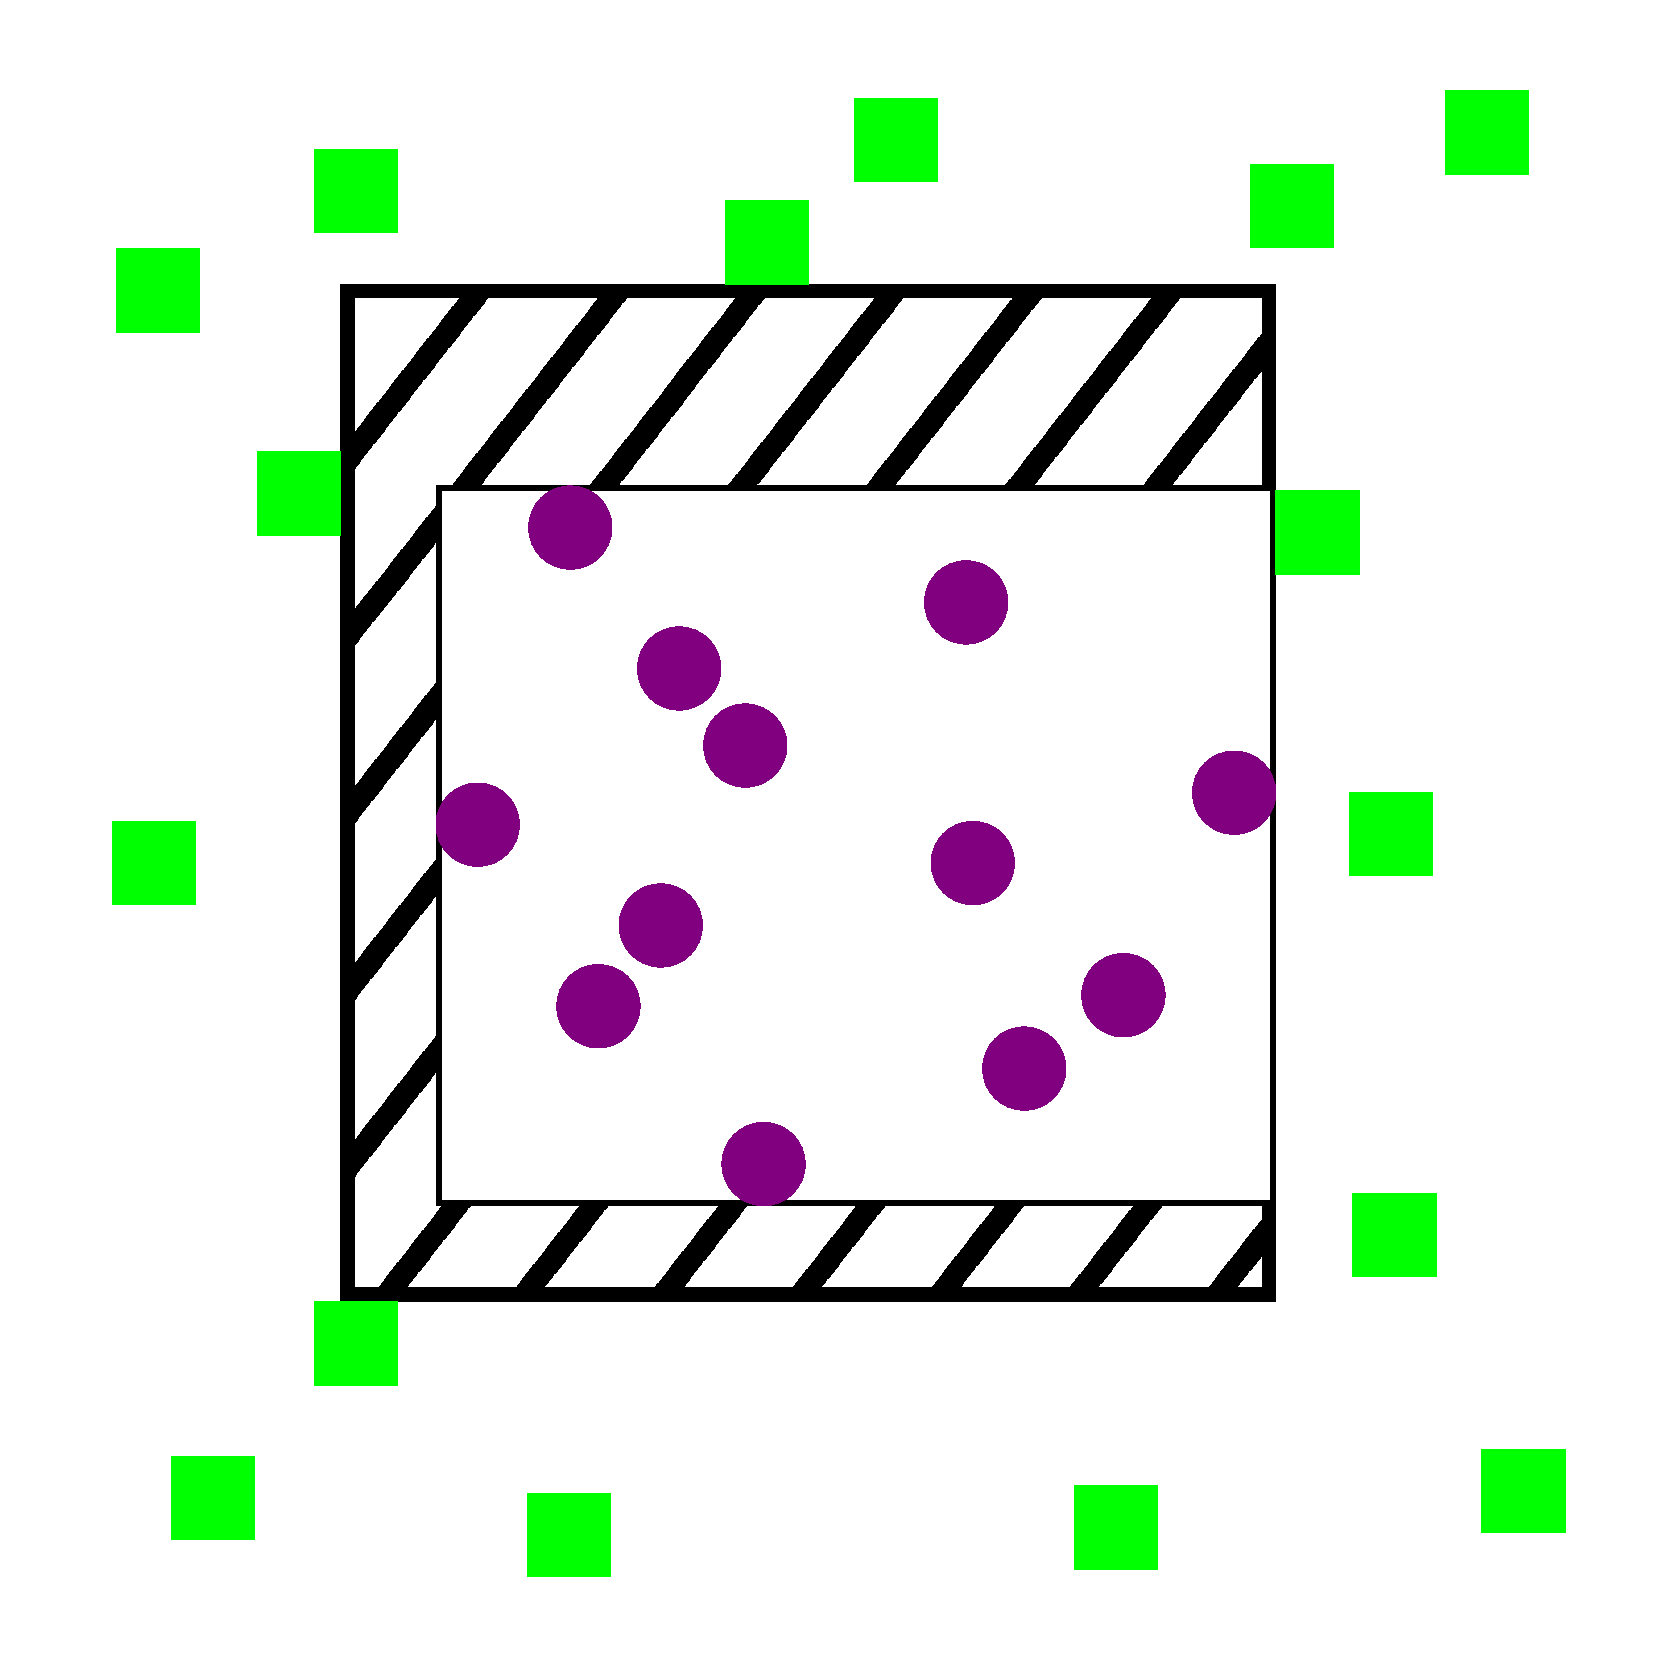
\includegraphics
      [width=0.5\textwidth,keepaspectratio]
      {boundary_choice}
      \caption{
        Проблема выбора границы
      }
      \label{fig:possiblities}
\end{figure}


\begin{enumerate}
\item Невозможно гарантировать получение наилучшего набора правил.
\item Получаемые правила зачастую нуждаются в упрощении.
\item Получаемые правила зачастую нуждаются в диверсификации
  \cite{voron10logicalgs}, \cite{vainzvaig75voting}.
\end{enumerate}

Избавиться от первой проблемы невозможно, с ней можно только бороться
с помощью различных эвристических алгоритмов. Для решения второй
проблемы существует большое число подходов, обзор можно посмотреть в
\cite{furnkranz97pruning}. Проблема диверсификации, наконец,
заключается в том, что довольно часто находятся очень похожие
закономерности. На примере из \cite{voron10logicalgs} можно понять,
почему это действительно плохо:

\begin{example}
  Предположим, что в некоторой экспертной комиссии есть два эксперта,
  мнения которых всегда (или почти всегда) совпадают по всем
  вопросам. Интуитивно понятно, что если убрать одного из экспертов,
  то качество работы новой комиссии будет таким же (или почти таким
  же).
\end{example}

\section{Обработка логических закономерностей}
\label{sec:processing}
%% Название этого раздела обязательно надо заменить на~содержательное.
%% В~этом разделе, как правило, много подразделов.

%% В~дипломной работе не~стоит делать более двух уровней, достаточно
%% разделов и~подразделов. Будете писать диссертацию или монографию~---
%% сделаете три уровня.

Для того, чтобы упростить и диверсифицировать полученное в результате
работы некоторого логического алгоритма классификации множества
логических закономерностей \(\varphi_1(x), \dots, \varphi_n(x)\),
предлагается провести его обработку с помощью дисперсионного критерия.
Основную схему этого подхода, предложенного В.~В.~Рязановым, можно
описать следующим образом:

\begin{enumerate}
\item Каждой логической закономерности \(\varphi_j^i\) из множества
  \(
  \mathcal{K}_{i} = \left\{
  \varphi_1^i(x), \dots, \varphi_t^i(x)
  \right\}
  \)
  логических закономерностей, покрывающих класс \(y_i\), поставить в
  соответствие некоторый вектор \(\bm{z}_j\), описывающий эту
  закономерность.
\item Провести кластеризацию векторов \(\bm{z}_1, \dots, \bm{z}_t\) на
  \(k \leq t\) кластеров и найти центры этих кластеров
  \(\bm{z}_1^*, \dots, \bm{z}_k^*\).
\item По центрам кластеров восстановить \(\varphi_1^*(x), \dots,
  \varphi_k^*(x)\) --- некоторые, вообще говоря новые, логические
  закономерности для класса \(y_i\).
\end{enumerate}

\subsection{Способы представления логических закономерностей}
\label{subsec:representation}
В этой работе рассмотрено два способа представить логические
закономерности: с помощью бинарного вектора и с помощью вектора левых
и правых границ.

Представление с помощью бинарного вектора было исследовано в
\cite{novikov15}. Идея заключается в том, чтобы каждой логической
закономерности \(\varphi(x)\) поставить в соответствие вектор
\(\bm{z}\in \left\{0, 1\right\}^l\) так, что

\[
\bm{z}_i =
\begin{dcases*}
1 & если \(\varphi(x_i) = 1\) \\
0 & иначе
\end{dcases*}
\]

В данной работе предлагается использовать представление с помощью
вектора левых и правых границ, которое использует введенное в
\ref{subsec:defs} представление логической закономерности
\(\varphi(x)\) в виде параметрических элементарных предикатов
(\ref{eq:parpred}). При таком подходе вектор \(\bm{z}\) принимает вид:

\[\bm{z} = (c_1^1, c_2^1, c_1^2, c_2^2, \dots, c_1^d, c_2^d)\]

\subsection{Алгоритм кластеризации логических закономерностей}
На этом шаге нужно разбить полученное описание множества логических
закономерностей \(\bm{z}_1, \bm{z}_2, \dots, \bm{z}_t\) на \(k \leq
t\) непересекающихся классов \(\bm{S} = \left\{S_1, S_2, \dots,
S_k\right\}\) таким образом, чтобы минимизировать функционал
\ref{eq:quality}. При этом для каждой закономерности предлагается
учитывать <<вес>>, то есть добавить константные коэффициенты
\(\beta_j\):

\begin{equation}\label{eq:quality}
\bm{S}^* =
\argmin_{\bm{S}}
\sum_{i=1}^k \sum_{\bm{z}_j\in S_i} \beta_j \|\bm{z}_j - \bm{\mu}_i\|^2
\end{equation}

Тогда алгоритм кластеризации
(алгоритм Ллойда \cite{lloyd06}, алгоритм К-средних \cite{macqueen67})
примет вид [\ref{algo:cluster}]

\begin{algorithm}[!htpb]
  \caption{Алгоритм кластеризации (Ллойда, К-средних)}
  \label{algo:cluster}
  \SetKwInOut{Input}{Вход}\SetKwInOut{Output}{Выход}
  \Input{Описание закономерностей \(\bm{z}_1, \dots, \bm{z}_t\)}
  \Output{
    \(\bm{S}^* =S_1, \dots, S_k\) --- разбиение на непересекающиеся
    кластеры
  }
  \SetKwFunction{IREP}{IREP}
  \SetKwProg{Fn}{Функция}{}{}
  \SetKwFor{While}{Пока}{}{}
  \SetKwIF{If}{Elif}{Else}{Если}{то}{Иначе если}{Иначе}{}
  \SetKw{KwRet}{Вернуть}
  \Fn{Кластеризовать(\(\bm{z}_1, \dots, \bm{z}_t\))} {
    Инициализировать центры кластеров
    \(\bm{\mu}_1^1, \dots, \bm{\mu}_k^1\)\;
    \While{кластеризация не стабилизируется}{
      \tcc{распределить объекты по кластерам, при этом}
      \tcc{минимизировать функционал качества(\ref{eq:quality})}
      \(
      S_i^t = \left\{
      \bm{z}_p : \beta_p \|\bm{z}_p - \bm{\mu}_i^t\|^2
      \leq
      \beta_p \|\bm{z}_p - \bm{\mu}_j^t\|^{2}, \forall j: 1\leq j\leq k
      \right\}
      \)\;
      \tcc{пересчитать центры кластеров с учетом веса}
      \(
      \bm{\mu}_i^{t+1} =
      \frac{1}{|S_i^t|}
      \frac{
        \sum_{\bm{z}_j\in S_i^t}\beta_j \bm{z}_j
      }{
        \sum_{\bm{z}_j\in S_i^t}\beta_j
      }
      \)\;
    }
    \KwRet{\(S_1^t, \dots, S_k^t\)}\;
  }
\end{algorithm}

\subsection{Восстановление логических закономерностей}
После того, как алгоритм кластеризации находит разбиение
\(\bm{S}^*\), необходимо по центрам кластеров
\(\bm{\hat{z}}_1^*, \dots, \bm{\hat{z}}_k^*\)
восстановить логические закономерности
\(\varphi_1^*(x), \dots, \varphi_k^*(x)\).

В случае, когда логические закономерности исходно были представлены в
виде бинарных векторов, полученный центр кластера \(\bm{\hat{z}}_i^*\)
уже, вообще говоря, не является бинарным вектором. Поэтому для каждого
вектора \(\bm{\hat{z}}^*_i, i = 1,\dots, k\) выбирается некоторый порог
бинаризации \(\theta_i\) таким образом, чтобы логическая закономерность
\(\varphi_i^*(x)\), отвечающая представлению:

\[
\bm{z}_i^* =
\begin{dcases*}
1 & если \(\bm{\hat{z}}_i^* \geq \theta_i\) \\
0 & иначе
\end{dcases*}
\]

была наиболее информативной среди всех рассмотренных значений порога
\(\theta_i\). Информативность логической закономерности рассчитывается
с помощью известных критериев информативности, таких как энтропийный
критерий IGain. Подробный обзор использования разных критериев для
этой задачи представлен в \cite{novikov15}.

В случае, когда логические закономерности исходно описывались с
помощью вектора левых и правых границ, полученный центр кластера
\(\bm{\hat{z}}_i^*\) можно использовать в качестве описания
\(\bm{z}_i^*\) некоторой новой логической закономерности. То есть нет
необходимости проводить отдельную процедуру по восстановлению
описания.

\section{Вычислительные эксперименты}
\label{sec:experiments}
%% Цель данного раздела: продемонстрировать, что предложенная теория
%% работает на практике; показать границы её применимости; рассказать
%% о~новых экспериментальных фактах.

Основной целью вычислительных экспериментов было реализовать подход
обработки множества логических закономерностей с помощью
дисперсионного критерия, описанного в разделе
\ref{sec:processing}. Также целью вычислительного эксперимента было
сравнить способы представления логических закономерностей, описанные в
разделе \ref{subsec:representation}. Для этого была принята следующая
схема проведения эксперимента:

\begin{enumerate}
  \item Исходная выборка делилась пополам на подвыборки обучения и
    контроля. При этом для подвыборок сохранялись одинаковые пропорции
    классов.
  \item На подвыборке обучения в системе <<Распознавание>>
    \cite{recognition06} настраивался классификатор <<логические
    закономерности>>.
  \item Логические закономерности настроенного классификатора
    импортировались в программу, реализующую дисперсионный подход в
    обработке логических закономерностей.
  \item По этому набору логических закономерностей с помощью
    алгоритма <<простого голосования>> \cite{voron10logicalgs}
    проводилась классификация контрольной подвыборки.
  \item Далее проводилось описание логических закономерностей одним из
    двух способов из раздела \ref{subsec:representation}. Полученные
    описания проходили кластеризацию на \(t = 2, 3, \dots, n, \dots\)
    кластеров.
  \item По полученным на очередном шаге \(t\) центрам кластеров
    восстанавливались новые логические закономерности, которые затем
    использовались в алгоритме <<простого голосования>> для
    классификации контрольной подвыборки.
  \item Полученные значения доли правильно классифицированных объектов
    для разных способов представления и для разного числа кластеров
    \(t\) выносилось на график.
\end{enumerate}

\subsection{Исходные данные и~условия эксперимента}
%% Описывается прикладная задача, параметры анализируемых данных
%% (например, сколько объектов, сколько признаков, каких они типов),
%% параметры эксперимента (например, как производился скользящий
%% контроль).

Исходные данные были взяты из репозитория UCI \cite{Lichman2013}.
Ниже представлена сводная таблица по использованным данным
[\ref{tab:data}]:

\begin{savenotes}
\begin{table}[!htbp]
  \begin{tabu}{X X X[2] X}
    Выборка & Объекты & Объекты по классам & Признаки \\ \hline
    Iris\footnotemark[1] & 150 & 50/50/50 & 4   \\
    Wine\footnotemark[2] & 178 & 59/71/48 & 13  \\
    Climate\footnotemark[3] & 540 & 46/494   & 11  \\
    Ionosphere\footnotemark[4] & 351 & 126/255  & 34  \\
  \end{tabu}
  \caption{Сводная таблица по использованным данным}
  \label{tab:data}
\end{table}
\end{savenotes}

Выборка Iris\footnotemark[1] ставит задачу классификации растений
семейства ирисов. Выборка Wine\footnotemark[2] содержит данные
химического анализа вина, полученного от трех разных итальянских
виноделов. Выборка Climate\footnotemark[3] содержит информацию об
удачных и неудачных запусках симулирования погоды. Наконец, выборка
Ionosphere\footnotemark[4] исследует свободные электроны в ионосфере.

\footnotetext[1]{\url{http://archive.ics.uci.edu/ml/datasets/Iris}}
\footnotetext[2]{\url{http://archive.ics.uci.edu/ml/datasets/Wine}}
\footnotetext[3]{
  \url{
    https://archive.ics.uci.edu/ml/datasets/Climate+Model+Simulation+Crashes
  }
}
\footnotetext[4]{\url{https://archive.ics.uci.edu/ml/datasets/Ionosphere}}


\subsection{Результаты эксперимента}
%% Результаты экспериментов представляются в~виде таблиц и~графиков.
%% Объясняется точный смысл всех обозначений на графиках, строк
%% и~столбцов в~таблицах.

Результаты запусков различных конфигураций метода обработки множества
логических закономерностей с помощью дисперсионного критерия
представлены на графиках \ref{fig:iris}, \ref{fig:wine},
\ref{fig:climate-new}, \ref{fig:climate-new2}, \ref{fig:ionosphere} и
\ref{fig:ionosphere2}. Сплошная линия красного цвета обозначает
качество классификации исходного множества логических
закономерностей. Синяя линия с кружками обозначает предложенный в
данной работе подход, зеленая линия с треугольниками и бирюзовая с
квадратами --- подходы с бинаризованным описанием и критериями
информативности IGain и Stat \cite{voron10logicalgs}.

Критерий информативности IGain --- это энтропийный критерий
информативности правила \(\varphi(x)\), отвечающего классу \(y_i\),
который имеет вид (\ref{eq:igain})

\begin{IEEEeqnarray}{rCl}\label{eq:igain}
\text{IGain} &=&
H\left(\frac{P}{P+N}, \frac{N}{P+N}\right)
- \frac{p + n}{P + N}
H\left(\frac{p}{p + n}, \frac{n}{p + n}\right) \nonumber \\
&-& \frac{P + N - p - n}{P + N}
H\left(\frac{P - p}{P + N - p - n}, \frac{N - n}{P + N - p - n}\right)
\end{IEEEeqnarray}

В формуле (\ref{eq:igain}) введено обозначение энтропии \(H(p, q) =
-p\log_2(p) -q\log_2(q)\), \(P, N\)~---~число объектов класса \(y_i\)
и не \(y_i\) соответственно, а \(p, n\)~---~число объектов из класса
\(y_i\) и не из класса \(y_i\), которые покрывает логическая
закономерность \(\varphi(x)\).

Критерий Stat имеет вид (\ref{eq:stat})

\begin{IEEEeqnarray}{rCl}\label{eq:stat}
  \text{Stat} &=&
  -\ln \frac{C_{P_1}^{p_1}\dots C_{P_K}^{p_K}}{C_l^{p_1 + \dots + p_K}}
  \end{IEEEeqnarray}

В формуле (\ref{eq:stat}) используется обозначение
\(P_1, \dots, P_K\) --- количество объектов в классе \(1, \dots, K\)
и \(p_1, \dots, p_K\) --- количество объектов класса, покрываемых
закономерностью \(\varphi(x)\). Наконец,
\(C_n^k = \frac{n!}{k! (n-k)!}\) обозначает биномиальный коэффициент.

\begin{figure}[!htbp]
  \centering
  \begin{subfigure}{0.8\textwidth}
  \centering
  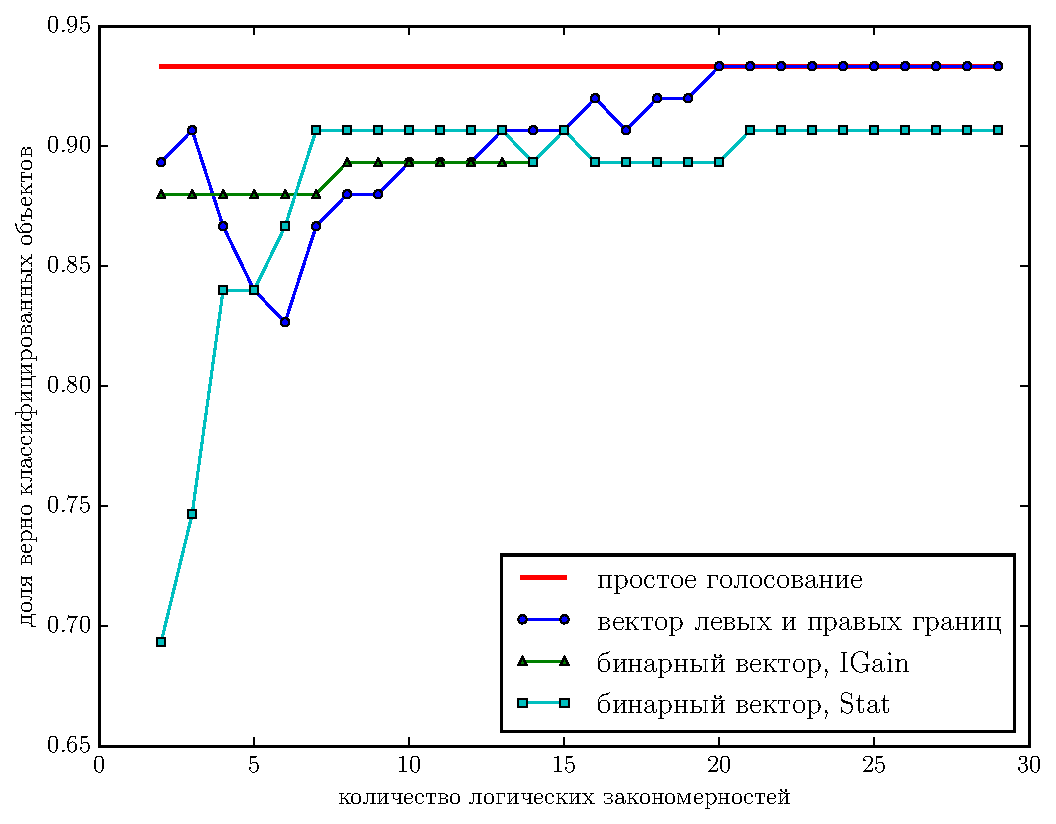
\includegraphics
      [width=\textwidth,keepaspectratio]
      {iris}
      \caption{
        Выборка Iris
      }
      \label{fig:iris}
  \end{subfigure}
  \begin{subfigure}{0.8\textwidth}
  \centering
  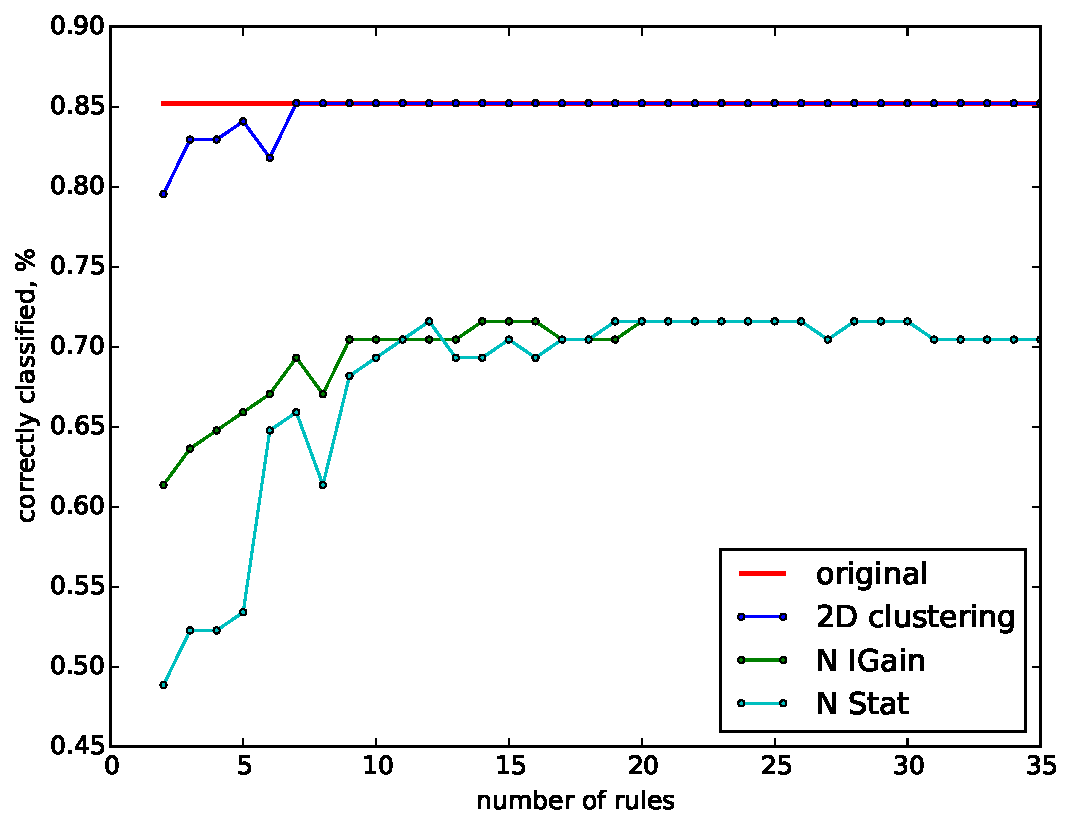
\includegraphics
      [width=\textwidth,keepaspectratio]
      {wine}
      \caption{
        Выборка Wine
      }
      \label{fig:wine}
  \end{subfigure}
\end{figure}

\begin{figure}
  \centering
  \begin{subfigure}{0.8\textwidth}
  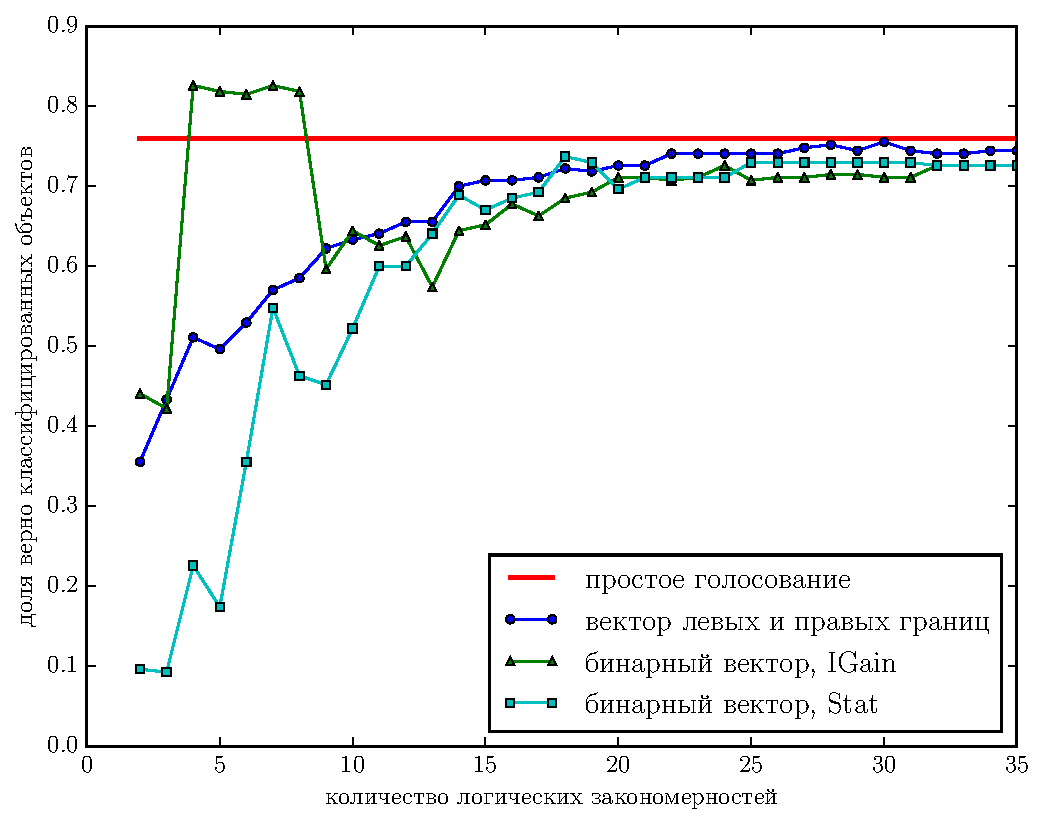
\includegraphics
      [width=\textwidth,keepaspectratio]
      {climate-new}
      \caption{
        Выборка Climate, исходные логические закономерности чистые (не
        покрывают объекты чужих классов)
      }
      \label{fig:climate-new}
  \end{subfigure}
  \begin{subfigure}{0.8\textwidth}
    \centering
    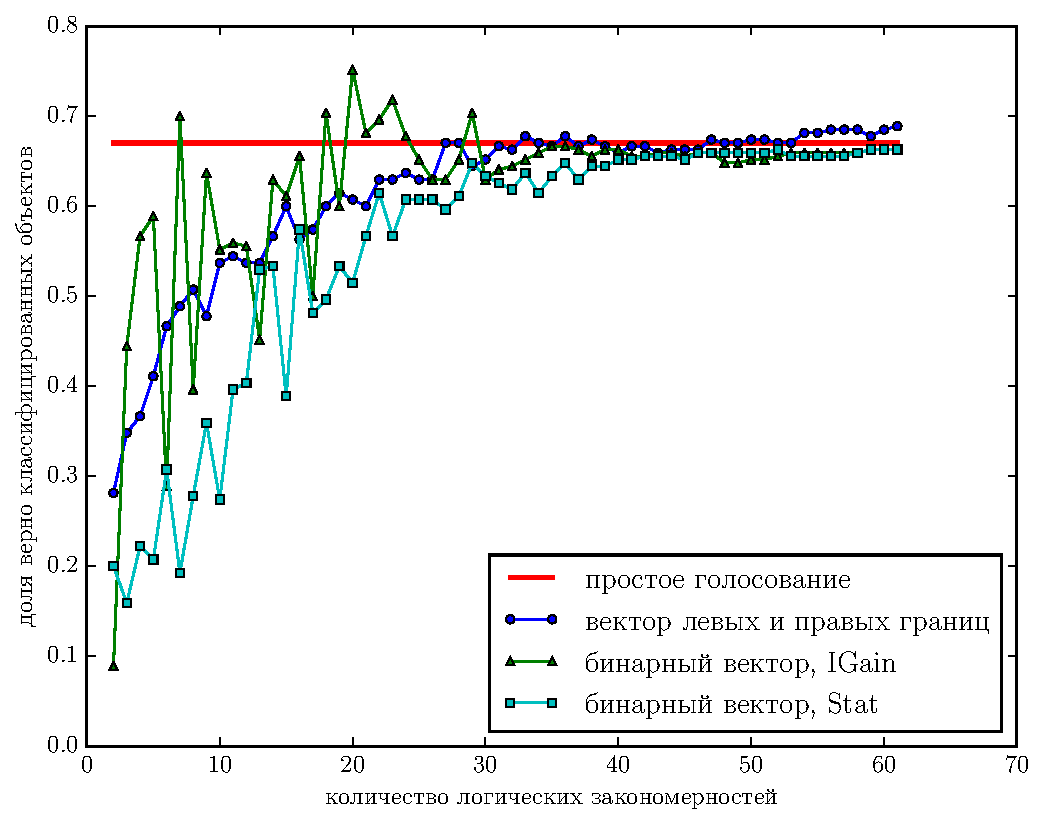
\includegraphics
      [width=\textwidth,keepaspectratio]
      {climate-new2}
      \caption{
        Выборка Climate, исходные логические закономерности частичные
        (среди покрываемых объектов не более 10\% из чужих классов)
      }
      \label{fig:climate-new2}
  \end{subfigure}
\end{figure}

\begin{figure}
  \centering
  \begin{subfigure}{0.8\textwidth}
  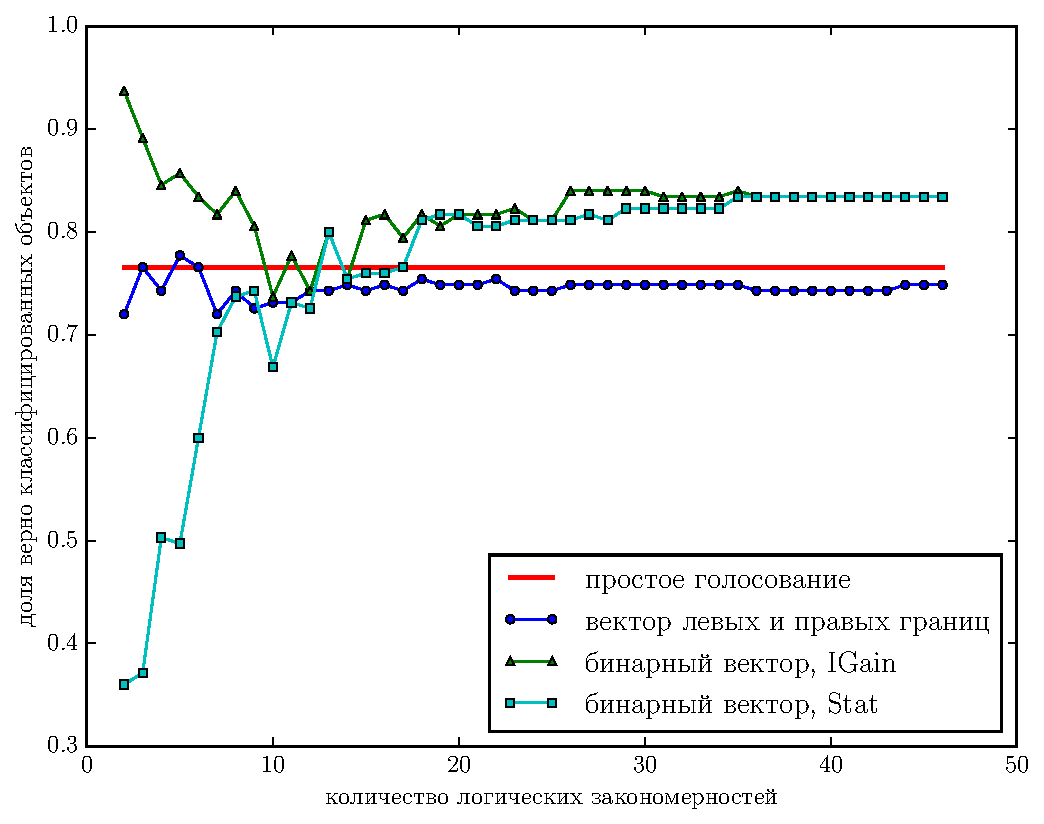
\includegraphics
      [width=\textwidth,keepaspectratio]
      {ionosphere}
      \caption{
        Выборка Ionosphere, исходные логические закономерности чистые
        (не покрывают объекты чужих классов)
      }
      \label{fig:ionosphere}
  \end{subfigure}
  \begin{subfigure}{0.8\textwidth}
    \centering
    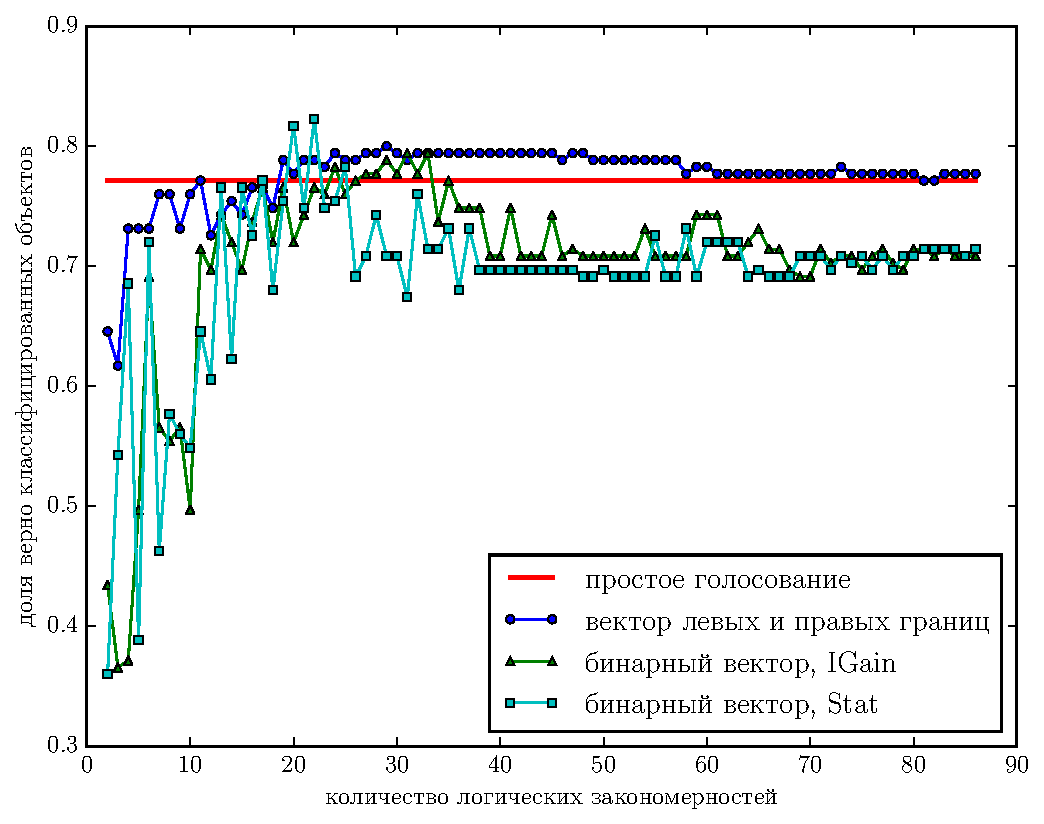
\includegraphics
      [width=\textwidth,keepaspectratio]
      {ionosphere2}
      \caption{
        Выборка Ionosphere, исходные логические закономерности
        частичные (среди покрываемых объектов не более 10\% из чужих
        классов)
      }
      \label{fig:ionosphere2}
  \end{subfigure}
\end{figure}

\subsection{Обсуждение и выводы}
%% Приводятся выводы: в~какой степени результаты экспериментов
%% согласуются с~теорией?  Достигнут ли желаемый результат?  Обнаружены
%% ли какие-либо факты, не~нашедшие объяснения, и~которые нельзя
%% списать на «грязный» эксперимент?

%% Обсуждаются основные отличия предложенных методов от известных
%% ранее. В~чем их преимущества? Каковы границы их применимости? Какие
%% проблемы удалось решить, а~какие остались открытыми?  Какие возникли
%% новые постановки задач?

\begin{itemize}
  \item Обработка логических закономерностей, использующая описание
    правил с помощью вектора левых и правых границ, получает
    результат, близкий к исходному набору логических закономерностей.
  \item Обработка логических закономерностей, использующая описание
    правил с помощью вектора левых и правых границ, восстанавливает
    логические закономерности, которые в целом показывают результаты
    лучше, чем результаты обработки с использованием бинаризованных
    описаний правил \ref{fig:iris}, \ref{fig:wine},
    \ref{fig:climate-new}, \ref{fig:climate-new2}.
  \item Обработка с использованием бинаризованных представлений правил
    иногда работает лучше \ref{fig:ionosphere}. Если же исходно
    используются не чистые, а частичные закономерности, то
    представление с помощью вектора левых и правых границ более
    устойчиво \ref{fig:climate-new2}, \ref{fig:ionosphere2}
  \item В результате обработки множества логических закономерностей
    как с помощью бинаризованного представления, так и с помощью
    вектора левых и правых границ, можно получить сравнимое с исходным
    качество классификации при меньшем количестве использованных
    правил.
\end{itemize}

\section{Заключение}

%% В~квалификационных работах последний раздел нужен для того, чтобы
%% конспективно перечислить основные результаты, полученные лично
%% автором.

%% Результатами, в~частности, являются:
%% \begin{itemize}
%% \item
%%     Предложен новый подход к\dots
%% \item
%%     Разработан новый метод\dots, позволяющий\dots
%% \item
%%     Доказан ряд теорем, подтверждающих (опровергающих), что\dots
%% \item
%%     Проведены вычислительные эксперименты\dots, которые подтвердили /
%%     опровергли / привели к~новым постановкам задач.
%% \end{itemize}

%% Цель данного раздела: доказать квалификацию автора.  Даже беглого
%% взгляда на заключение должно быть достаточно, чтобы стало ясно:
%% автору удалось решить актуальную, трудную, ранее не~решённую задачу,
%% предложенные автором решения обоснованы и~проверены.

%% Иногда в~Заключении приводится список направлений дальнейших
%% исследований.

В данной работе был предложен подход к обработке множеств логических
закономерностей. В частности, в разделе \ref{sec:processing} была
сформулирована схема использования дисперсионного критерия, а в
разделе \ref{sec:experiments} были поставлены эксперименты по
исследованию этого подхода. С их помощью удалось сравнить
использование бинаризованного описания логических закономерностей,
предложенное в \cite{novikov15}, и описание логических закономерностей
с помощью вектора левых и правых границ, предложенное в данной работе.
В результате предложенный в данной работе подход с использованием
вектора левых и правых границ и взвешенной кластеризации в целом
работает лучше, чем подход с бинаризованным описанием. Качество
классификации сравнимо с исходным алгоритмом системы
<<Распознавание>>, но при этом размер множества логических
закономерностей меньше.

\newpage
%% Список литературы необходим в~любой научной публикации. В дипломной
%% работе он~обязателен. Дурным тоном считается: ссылаться на работы
%% только одного-двух авторов (например, себя или шефа); ссылаться на
%% слишком малое число работ; ссылаться только на очень старые работы;
%% ссылаться на работы, которых автор ни разу не видел; ссылаться
%% на~работы, которые не~упоминаются в~тексте или которые не~имеют
%% отношения к~данному тексту.

\appendix
\section{Система <<Распознавание>>}
Система <<Распознавание>> \cite{recognition06} работает под
управлением операционной системы семейства Microsoft Windows XP и
выше. В этом приложении будет показано, как систему <<Распознавание>>
можно использовать на UNIX-подобных операционных системах. Для этого
нужно:

\begin{enumerate}
  \item Установить свободное программное обеспечение
    \href{https://www.winehq.org/}{Wine}.
  \item Настроить 32-битный префикс командой
    \mint{shell}|WINEARCH=win32 WINEPREFIX=~/.wine32 winecfg|
  \item Установить в созданный префикс недостающую библиотеку
    \mint{shell}|WINEPREFIX=~/.wine32 winetricks mfc42|
  \item Запустить систему <<Распознавание>> командой
    \begin{minted}{shell}
      LC_CTYPE=ru_RU.utf8 WINEARCH=win32 WINEPREFIX=~/.wine32 \
      wine Recognition.exe
    \end{minted}
\end{enumerate}

\section{Формат файлов *.tab}

Система <<Распознавание>> \cite{recognition06} использует собственный
формат файлов описания выборки. Здесь приведено описание этого
формата:

Первая строка --- заголовок. Представляет из себя числа, разделенные
пробелом. Первое число --- количество признаков каждого объекта
выборки. Второе --- количество классов. Далее идет число \(0\), за
которым идет число объектов первого класса, затем сумма числа объектов
первых двух классов, затем сумма числа объектов первых трех классов и
так далее. Завершает заголовок число, обозначающее пропуск измерения в
данных.

Каждая последующая строка содержит признаковое описание отдельного
объекта, разные классы разделены пустой строкой.

\printbibliography

\end{document}
